\section{Programming in Python}
\label{app:Python}
Most of the content in the guide comes from the documentation, available online \href{https://sourceforge.net/p/raspberry-gpio-python/wiki/Home/}{here}.

Python, while not as powerful as C or C++, is quickly becoming a common choice for embedded systems developers due to its ease of use and rapid development times\footnote{See \href{https://spectrum.ieee.org/at-work/innovation/the-2018-top-programming-languages}{https://spectrum.ieee.org/at-work/innovation/the-2018-top-programming-languages}}. 

This chapter serves as a short guide for programming in Python on the RPi. You will also find some templates for techniques such as debouncing, or making use of the Raspberry Pi's multicore architecture by implementing threading.

\subsection{The RPI.GPIO Library}
The RPi.GPIO library is the common Python library used on the Raspberry Pi. 
Documentation for the library can be found here:\\
\href{https://sourceforge.net/p/raspberry-gpio-python/wiki/Home/}{https://sourceforge.net/p/raspberry-gpio-python/wiki/Home/}

It is included in the environment variables by default, so to use it, you can simply just import it into your Python script:

\begin{lstlisting}
include RPi.GPIO as GPIO
\end{lstlisting}

You need to specify which board mode you're using. For more information on board modes, see Section \ref{sec:BoardModes}. Board modes are specified as follows:
\begin{lstlisting}
GPIO.setmode(GPIO.BOARD)
# or
GPIO.setmode(GPIO.BCM)
\end{lstlisting}

You also need to perform "cleanup" on GPIOs when your application exists. By performing cleanup and resetting all pins to their default modes, you can prevent possible damage to your Raspberry Pi. The cleanup function is called as follows:
\begin{lstlisting}
GPIO.cleanup()
\end{lstlisting}

If your program is meant to run indefinitely, and only close upon an exception, you can wrap it in a try catch, as follows:
\begin{lstlisting}
if __name__ == "__main__":
	# Make sure the GPIO is stopped correctly
	try:
	    while True:
		    main()
	except KeyboardInterrupt:
		print("Exiting gracefully")
		GPIO.cleanup()
	except e:
		print("Some other error occurred: {}".format(e.message)})
		GPIO.cleanup()
\end{lstlisting}


\subsection{Basic IO}
Read the documentation, available \href{https://sourceforge.net/p/raspberry-gpio-python/wiki/Outputs/}{here}.

\subsubsection{Digital Logic}
Digital output on the Raspberry Pi is accomplished by writing values to channels. A channel is a pin, which is numbered in the way you've configured. 
Basic configuration of a pin for output is as follows:
\begin{lstlisting}
GPIO.output(<channel>, <Logic>)
\end{lstlisting}
Your logic (high, 3.3V, or low, 0V), can be specified as follows:
\begin{itemize}
    \item For 3.3V (high) output:
        \begin{lstlisting}[gobble=12]
            GPIO.output(<channel>, GPIO.HIGH)
            GPIO.output(<channel>, 1)
            GPIO.output(<channel>, True)
        \end{lstlisting}
    \item For 0V (low) output:
    \begin{lstlisting}[gobble=12]
            GPIO.output(<channel>, GPIO.LOW)
            GPIO.output(<channel>, 0)
            GPIO.output(<channel>, False)
        \end{lstlisting}
\end{itemize}

Channels can also be specified in lists, for example:
\begin{lstlisting}
LEDs = (11,12)
GPIO.output(LEDs, GPIO.HIGH) # Will turn all channels HIGH
GPIO.output(LEDs, (GPIO.HIGH, GPIO.LOW)) # Will the first channel HIGH, and the second LOW
\end{lstlisting}

Note that you can also read the state of the pin/channel that is set as an output by using the \verb|input()| function. For example, if you wanted to toggle pin 12, you could do something as follows:
\begin{lstlisting}
GPIO.output(12, not GPIO.input(12))
\end{lstlisting}


\subsubsection{Analog}
The Raspberry Pi does not have any analog input pins. You will need to use something like the \href{https://cdn-shop.adafruit.com/datasheets/MCP3008.pdf}{MCP3008} to read analog voltages.


\subsubsection{Inputs}
\paragraph{Digital Read}
To read the value of a digital pin, you can use the \verb|input()| function:
\begin{lstlisting}
if GPIO.input(12):
    print("Pin 12 HIGH")
else:
    print("Pin 12 LOW")
\end{lstlisting}

\paragraph{Pull Up/Pull Down Resistors}
Using pull up and pull down resistors is essential when working with digital logic. Thankfully, the Raspberry Pi has internal pull up and pull down resistors. To make use of these, initialize the pin/channel as follows:
\begin{lstlisting}
GPIO.setup(<channel>, GPIO.IN, pull_up_down=GPIO.PUD_UP)
# or
GPIO.setup(<channel>, GPIO.IN, pull_up_down=GPIO.PUD_DOWN)
\end{lstlisting}

\paragraph{Interrupts} 
Very often it is useful to set up an interrupt, for example to trigger an event when a button is pressed. Callback functions are executed on a different thread. If you have multiple callbacks, know that they will be executed sequentially as only one thread exists for interrupts. Interrupts can be implemented as follows:
\begin{lstlisting}
# The bounce time is given in milliseconds.
# If your pin is set to use pull down resistors
# Connect a button between <channel> and 3.3V
GPIO.add_event_detect(<channel>, GPIO.RISING, callback=callback_method(), bouncetime=200)
# If your pin is set to use pull up resistors
# Connect a button between <channel> and GND
GPIO.add_event_detect(<channel>, GPIO.FALLING, callback=callback_method(), bouncetime=200)  
\end{lstlisting}

\paragraph{Other functions}
The RPi.GPIO Library offers other functions for interrupts the first is the \verb|wait_for_edge()| function, which is designed to block execution until an edge is detected. You can detect edges of \verb|GPIO.RISING|, \verb|GPIO.FALLING|, or \verb|GPIO.BOTH|. The timeout is given in milliseconds:
\begin{lstlisting}
# wait for up to 5 seconds for a rising edge
pin = GPIO.wait_for_edge(<channel>, GPIO_RISING, timeout=5000)
if pin is None:
    print('Timeout occurred')
else:
    print('Edge detected on pin ', pin)
\end{lstlisting}

Another function is the \verb|event_detected()| function. From the docs: "The event\_detected() function is designed to be used in a loop with other things, but unlike polling it is not going to miss the change in state of an input while the CPU is busy working on other things. This could be useful when using something like Pygame or PyQt where there is a main loop listening and responding to GUI events in a timely basis."

\begin{lstlisting}
GPIO.add_event_detect(channel, GPIO.RISING)  # add rising edge detection on a channel
do_something()
if GPIO.event_detected(channel):
    print('Button pressed')
\end{lstlisting}

\subsection{Communication Protocols}
The RPi.GPIO library has no native support for communication protocols. Very often, specific Python libraries are provided on a per-device use case. However, this can become tedious and cause your code to become bloated. See the sections below for relevant libraries for using I2C and SPI directly.

\subsubsection{I2C}
Ensure you enable I2C in \verb|raspi-config|.

To use I2C in Python, you can use the \verb|smbus| library. To do this, we need to install and configure smbus. This is usually done by default, but instructions are included for posterity.

\begin{lstlisting}
$ sudo apt-get install i2c-tools
$ sudo apt-get install python-smbus
$ sudo adduser <username> i2c
$ sudo reboot
\end{lstlisting}

Once you connect a device, you can run \verb|$gpio i2cdetect| to determine if a device is detected on the I2C bus. In the example below, there is an electronic compass (GY-271) connected to the Pi.
\begin{figure}[H]
\centering
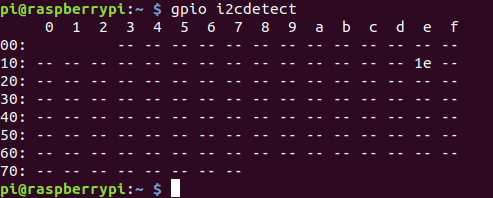
\includegraphics[width=0.7\columnwidth]{Figures/i2cdetect}
\caption{An i2cdetect example}
\label{fig:i2cdetect}
\end{figure}

To initialize an I2C device, do the following:
\begin{lstlisting}
import smbus
bus = smbus.SMBus(1) # 1 indicates /dev/i2c-1
address = 0x1e #whatever the device is for your i2c device
\end{lstlisting}

To read a byte from the I2C device:
\begin{lstlisting}
result = bus.read_byte_data(address, <register>)
\end{lstlisting}

To write a byte to the I2C device:
\begin{lstlisting}
bus.write_byte_data(address, <register>, <value>)
\end{lstlisting}

\paragraph{Methods Available}
\verb|smbus| has multiple methods. The documentation for these is quite minimal, but brief descriptions are available \href{http://wiki.erazor-zone.de/wiki:linux:python:smbus:doc}{here}.

\subsubsection{SPI}
Ensure you enable SPI in \verb|raspi-config|.

You can use SPI in Python by using the \verb|spidev| library. Documentation is available \href{https://pypi.org/project/spidev/}{here}. Basic usage is as follows:
\begin{lstlisting}
import spidev

#Bus is 0 or 1, depending on which SPI bus you've connected to
bus = 0
#Device is the chip select pin. Set to 0 or 1, depending on the connections
device = 1

spi = spidev.SpiDev() #Enable SPI
spi.open(bus, device) #Open connection to a specific bus and device (CS pin)

# Set settings (SPI speed and mode)
spi.max_speed_hz = 500000
spi.mode = 0

to_send = [0x01, 0x02, 0x03] #define what to send
spi.xfer(to_send)

# Close the SPI connection
close()
\end{lstlisting}

\paragraph{Settings}
The following settings are configurable in the \verb|spidev| library, and can be set as follows:
\begin{lstlisting}
spi = spidev.SpiDev() #Enable SPI
spi.<setting> = <value>
\end{lstlisting}
List of settings:
\begin{itemize}
    \item \verb|bits_per_word|
    \item \verb|cs_high|
    \item \verb|loop|\\
        Set the "SPI\_LOOP" flag to enable loopback mode
    \item \verb|no_cs|\\
        Set the "SPI\_NO\_CS" flag to disable use of the chip select (although the driver may still own the CS pin)
    \item \verb|lsbfirst|
    \item \verb|max_speed_hz|
    \item \verb|mode|\\
        SPI mode as two bit pattern of clock polarity and phase [CPOL/CPHA], min: 0b00 = 0, max: 0b11 = 3
    \item \verb|threewire|\\
        SI/SO signals shared
\end{itemize}

\paragraph{Methods}
The following methods are available in the \verb|spidev| library
\begin{itemize}
    \item \verb|open(bus, device)|\\
    Connects to the specified SPI device, opening \verb|/dev/spidev<bus>.<device>|
    \item \verb|readbytes(n)|\\
    Read n bytes from SPI device.
    \item \verb|writebytes(list of values)|\\
    Writes a list of values to SPI device.
    \item \verb|writebytes2(list of values)|\\
    Similar to `writebytes` but accepts arbitrary large lists. If list size exceeds buffer size (which is read from \verb|/sys/module/spidev/parameters/bufsiz|), data will be split into smaller chunks and sent in multiple operations.
    Also, writebytes2 understands \href{https://docs.python.org/3/c-api/buffer.html}{buffer protocol} so it can accept numpy byte arrays for example without need to convert them with \verb|tolist()| first. This offers much better performance where you need to transfer frames to SPI-connected displays for instance.
    \item \verb|xfer(list of values[, speed_hz, delay_usec, bits_per_word])|\\
    Performs an SPI transaction. Chip-select should be released and reactivated between blocks. Delay specifies the delay in usec between blocks.
    \item \verb|xfer2(list of values[, speed_hz, delay_usec, bits_per_word])|\\
    Performs an SPI transaction. Chip-select should be held active between blocks.
    \item \verb|xfer3(list of values[, speed_hz, delay_usec, bits_per_word])|\\
    Similar to xfer2 but accepts arbitrary large lists. If list size exceeds buffer size (which is read from \verb|/sys/module/spidev/parameters/bufsiz|), data will be split into smaller chunks and sent in multiple operations.
    \item \verb|close()|\\
    Disconnects from the SPI device.
\end{itemize}

\subsection{Using Threads}
\href{https://realpython.com/intro-to-python-threading/}{This guide} serves as the basis for the text below. This manual does not teach everything there is to know about threading in Python, but will give you the basics to be able to utilize threads for simple tasks that may be of use to you in the practicals. It's strongly recommended you read through that text if you have not yet been exposed to threading concepts.

This text does not cover issues and precautions when working with threads, such as mutex's and locks, data races, producer/consumer concerns and the likes. However, these are knowledge areas of critical importance, and it is strongly suggested that the reader tries to make an effort to understand these concerns before writing threaded code.

\subsubsection{The Threading Library}
The Python library \verb|threading| library offers all the functionality one would expect. Import it in to your code in the standard way:
\begin{lstlisting}
import threading
\end{lstlisting}

There are 4 basic things you need to do when creating a thread:
\begin{enumerate}
    \item Initialize it
    \item Start it
    \item Let is execute
    \item "Shut it down" by joining
\end{enumerate}

\subsubsection{Basic Thread Usage}
For example, if you want to create a separate thread to fetch a sensor value five times, you could do it as follows:
\begin{lstlisting}
import threading
import time
import RPi.GPIO as GPIO

def setup():
    #Contains all code for initialisation of RPi.GPIO

def fetch_sensor_vals(sensor_pin):
    for i in range 5:
        GPIO.input(sensor_pin)
        time.sleep(2)
    
if __name__ == "__main__":
    setup()
    # Create a thread to call the function and pass "12" in as sensor pin
    x = threading.Thread(target=fetch_sensor_vals, args=(12,)) 
    print("Starting thread")
    x.start()
    print("Waiting for the thread to finish")
    x.join()
    print("Reading finished")
\end{lstlisting}

\subsubsection{Timed Thread Usage}
Often in embedded systems we want a specific task to run every X time units. There is an option in the Python threading library. It works as follows:

\begin{lstlisting}
import threading
import datetime

"""
This function prints the time to the screen every five seconds
"""
def print_time():
    t = threading.Timer(5.0, print_time)
    t.daemon = True
    t.start()
    print(datetime.datetime.now())
	

if __name__ == "__main__":
    print_time() # call it once to start the thread
    
    # Tell our program to run indefinitely
    while True:
        pass
\end{lstlisting}

You will see that in this code example, we have also set the \verb|daemon| flag of the thread to be be \verb|True|. A daemon thread will shut down immediately when the program exits. In essence, the daemon thread will run indefinitely in the background until your application exits, and you do not need to worry about calling \verb|join()|.\footnote{It's important to note that calling t.join() will wait for a thread to finish executing, even if it is a daemon.}